\documentclass[a4,center,fleqn]{NAR}


\usepackage{NAR-natbib}
\bibliographystyle{NAR-natbib}
\usepackage{color}
\usepackage{xfrac}
\newcommand{\rngcomment}[1]{{\color{red}RNG: #1}}
\newcommand{\bkmcomment}[1]{{\color{blue}BKM: #1}}
\newcommand{\batcave}{BATCAVE }
\newcommand{\beginsupplement}{%
        \clearpage
        \onecolumn
        \setcounter{table}{0}
        \renewcommand{\thetable}{S\arabic{table}}%
        \setcounter{figure}{0}
        \renewcommand{\thefigure}{S\arabic{figure}}%
     }
% Enter dates of publication
\copyrightyear{2008}
\pubdate{31 July 2009}
\pubyear{2009}
\jvolume{37}
\jissue{12}

\articlesubtype{Genomics and Bioinformatics}

\begin{document}

\title{\batcave: Bayesian Analysis Tools for Context-Aware Variant Evaluation}

\author{%
Brian K. Mannakee\,$^{1}$ and
Ryan N. Gutenkunst\,$^{2}$%
\footnote{To whom correspondence should be addressed.
Email: rgutenk@email.arizona.edu}}

\address{%
$^{1}$Mel and Enid Zuckerman College of Public Health, University of Arizona, Tucson AZ
and
$^{2}$Department of Molecular and Cellular Biology, University of Arizona, Tucson AZ}
% Affiliation must include:
% Department name, institution name, full road and district address,
% state, Zip or postal code, country

\history{%
Received January 1, 2009;
Revised February 1, 2009;
Accepted March 1, 2009}

\maketitle

\begin{abstract}
Text. Text. Text. Text. Text. Text. Text. Text. Text. Text. Text.
Text. Text. Text. Text. Text. Text. Text. Text. Text. Text. Text.
Text. Text. Text. Text. Text. Text. Text. Text. Text. Text. Text.
Text. Text. Text. Text. Text. Text. Text. Text. Text. Text. Text.
Text. Text. Text. Text. Text. Text. Text. Text. Text. Text. Text.
Text. Text. Text. Text. Text. Text. Text. Text. Text. Text. Text.
Text. Text. Text. Text. Text. Text. Text. Text. Text. Text. Text.
Text. Text. Text. Text. Text. Text. Text. Text. Text. Text. Text.
Text. Text.
\end{abstract}


\section{Introduction}

Cancer develops as the result of the accumulation of somatic mutations and clonal selection of cells with mutations that confer a selective advantage on the cell.
Understanding the forces that shaped the evolutionary history of a tumor, the mutations that are responsible for its growth, the rate at which mutations are occurring, or how much genetic diversity is likely present in the tumor, requires accurate variant calling, particularly at low variant allele frequency \cite{Williams2016,Bozic2016,Williams2018,Shi2018}.
Accurate variant identification is also critical in optimizing the treatment regime for an individual patients disease \citep{Ding2012,Mardis2012,Chen2013,Borad2014,Findlay2016}.
Low frequency mutations present a significant problem for current mutation calling methods because their signature in the data is difficult to distinguish from the noise introduced by Next Generation Sequencing (NGS), and this problem increases as sequencing depth increases.

Methods for identifying true somatic mutations - i.e. variant calling -  from NGS data are an active area of research in bioinformatics.
The earliest widely used somatic variant callers aimed specifically at tumors, Mutect1 and Varscan2, used a combination of heuristic filtering and a model of sequencing errors to identify and score potential variants, setting a threshold for that score designed to balance sensitivity and specificity \citep{Koboldt2012,Cibulskis2013}.
Subsequent research gave rise to a number of alternate variant calling strategies including haplotype based callers \citep{Garrison2012},
joint genotype analysis (SomaticSniper, JointSNVMix2, Seurat, and CaVEMan,MuClone)\citep{Larson2012,Roth2012a,Christoforides2013,Jones2016,Dorri2019}, allele frequency based analysis (Strelka, MuTect, LoFreq, EBCall, deepSNV, LoLoPicker, and MuSE)\citep{Saunders2012,Wilm2012,Shiraishi2013b,Gerstung2012,Carrot-Zhang2017,Fan2016}, and a mixture of ensemble and deep learning methods (MutationSeq, SomaticSeq, SNooPer, and BAYSIC).
All of these methods have varying levels of complexity, and some are focused on specific types of data.
The one thing they all have in common is that they either implicitly or explicitly assume that the probability of a mutation occuring at a particular site is proportional to the overall mutation rate, and the same at every site in the genome.

Single nucleotide variants (SNV) arise in tumors at a rate and at genomic locations driven by two main processes. 
The first is the spontaneous accumulation of mutations that occurs in all dividing tissues, and has a characteristic mutation signature that describes the probability of mutation in a given genomic context \citep{Nik-Zainal2012a,Alexandrov2015,Lee-Six2018}. 
The second -- and far more complex -- process is the accumulation of mutations through exposure to mutagens or degradation - via mutation or deletion - of cellular machinery responsible for the identification and repair of damage or replication errors. 
Many mutagens and DNA repair mechanism defects also have highly specific mutation signatures, such that they can be identified by observing the mutations in the tumor \citep{Alexandrov2013a,Helleday2014a,Nik-Zainal2016,Kandoth2013,Alexandrov2016}.
The specific processes driving mutations in a particular tumor generate a tumor's unique mutation profile, and differences within and between tumor types are pronounced \cite{Stephens2005, Burrell2013a, Nakamura2015, Witkiewicz2015, Kumar2016}
Figure \ref{NAR-sigfig} \textbf{a-e} shows several examples of mutation profiles from both real and simulated tumors.


Here we present an algorithm for estimating the prior probability of mutation at a given site using the observed mutation spectrum of the tumor as well as its mutation rate, and show that the addition of this prior to the MuTect variant calling model produces a superior variant classifier in both simulated and real tumor data.
We provide a simple implementation in R that takes MuTect caller output as input, and returns the posterior probability that a site is variant for every site observed by MuTect. \bkmcomment{batcave,batcaver,batcaveR}

\begin{figure}
  \begin{center}
  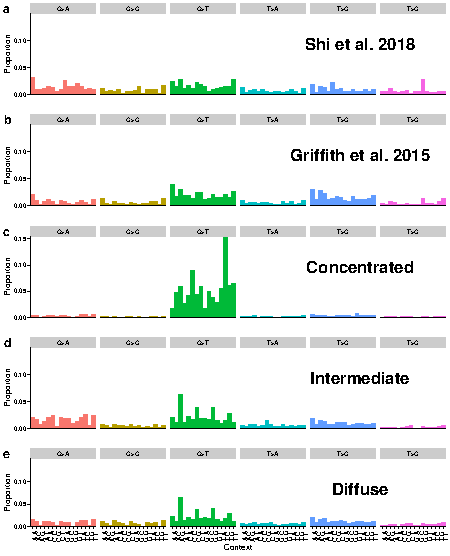
\includegraphics{figures/signatures_only.pdf}
  \end{center}
  \caption{Mutation profiles. 
  \textbf{(a)} The observed mutation profile of a breast cancer sample from \cite{Shi2018}.
  \textbf{(b)} The observed mutation profile of the AML 31 primary tumor from \cite{Griffith2015}.
  \textbf{(c)} A mutation profile used for simulating tumors, made up of equal proportions of COSMIC mutation signatures 1, 7, \& 11.
  \textbf{(d)} Equal proportions of signatures 1, 4, \& 5.
  \textbf{(e)} Equal proportions of signatures 1, 3, \& 5.
  }
  \label{NAR-sigfig}
  \end{figure}

\section{MATERIALS AND METHODS}
\subsection{Somatic variant calling base probability model}

At every site in the genome with non-zero coverage, Next Generation Sequencing (NGS) produces a vector \bkmcomment{push equation onto separate line} $\mathbf{x}  = (\{b_i\},\{q_i\}), i = 1\dots \mathrm{d}$ of base calls and their associated quality scores, where $\mathrm{d}$ is total read depth.
We want to use $\mathbf{x}$ to select between competing hypotheses;
\begin{equation}
  \label{eqn:hypothesis}
$$
  \begin{array}{l}
    \mathbf{H_0}:\quad \textrm{Alt allele} = m;\quad\nu = 0\\
    \mathbf{H_1}:\quad \textrm{Alt allele} = m;\quad\nu = \hat{f},
  \end{array}
$$
\end{equation}
where $\nu$ is the variant allele frequency, $\hat{f}$ is the maximum likelihood estimate of $\nu$ given data $\mathbf{x}$, i.e. the ratio of the count of variant reads and total read depth, and $m$ is any of the 3 possible alternate non-reference bases.
The posterior probability of a given hypothesis, $\mathrm{P}(m,\nu)$, is the product of the likelihood of the data given the hypothesis and the prior probability of the hypothesis. 
Assuming that reads are independent, we have

\begin{equation}
  \label{eqn:1}
$$
  \mathrm{P}(m,\nu) = \mathrm{p}(m,\nu) \cdot \prod_{i=1}^{\mathrm{d}} \textrm{f}_{m,\nu}(x_i),
$$
\end{equation}
where the density $\textrm{f}_{m,\nu}(x_i)$ can take several forms.

Assuming that the identity of the alternate allele and its allele frequency are independent of each other, and $\nu$ is uniformly distributed (i.e. $\mathrm{p}(\nu) = 1$), we can rewrite equation \ref{eqn:1} as
\begin{equation}
  \label{eqn:2}
$$
  \mathrm{P}(m,\nu) = \mathrm{p}(m) \cdot \prod_{i=1}^{\mathrm{d}} \textrm{f}_{m,\nu}(x_i).
$$
\end{equation}
Here we show how \batcave can be used to provide a tumor and site-specific estimate of the prior probability of mutation $\mathrm{p}(m)$.

\subsection{Site-specific prior probability of mutation}
The probability which we have denoted $\mathrm{p}(m)$ in equation \ref{eqn:2} for compactness is more precisely the joint probability that a mutation has occured $M$, and that it was to allele $m$, which we will denote here $\mathrm{p}(m,M)$.
However, $\mathrm{p}(m,M)$ is not constant for every site in the genome, and follows a distribution conditional on the genomic context surrounding the site, denoted here $\mathrm{p}(m,M | C)$ \cite{Buisson2019}.
Assuming that $m$ and $M$ are independent conditional on the genomic context, $\mathrm{p}(m,M \mid C) = \mathrm{p}(m \mid C) \mathrm{p}(M \mid C)$, which we can use Bayes' rule to further decompose as 

\begin{equation}
  \label{eqn:full_prior}
  $$
  \mathrm{p}(m,M \mid C) = \mathrm{p}(m \mid C) \mathrm{p}(C \mid M)\frac{\mathrm{p}(M)}{\mathrm{p}(C)}.
  $$
\end{equation}
We next show how to estimate the quantities in equation \ref{eqn:full_prior}.

\subsection{Estimation of the mutation profile}
There are many aspects of genomic architecture which can affect the somatic mutation rate at multiple scales \cite{Buisson2019}.
Here we focus on a small-scale feature, the tri-nucleotide context, which has been shown to have a strong effect on the prior probability of mutation \citep{Nik-Zainal2012a,Alexandrov2015,Lee-Six2018}.
The tri-nucleotide context at a particular genomic site is made up of the identity of the reference base and the identity of the 3` and 5` flanking bases.
There are four possible bases {\{A,C,T,G\}} 3` and 5` of the site, leading to 16 possible flanking base combinations.
Folding the central bases to the pyrimidines leaves 2 possible reference bases at the site {\{C,T\}}, resulting in $2 \cdot 16 = 32$ possible tri-nucleotide contexts.
We define a mutation context $C$ indexed by $c=\{1 \dots 32\}$, to be the tri-nucleotide context of a particular site in the genome. 
For each context, a mutation can be to any of the three possible alternate alleles {\{A,(C/T),G\}}. 
We can thus define $\mathrm{S}$, the substitution type, indexed by $c=\{1 \dots 32\}$ contexts and $m = \{1 \dots 3\}$ alternate bases, resulting in 96 possible substitution types.
Using the substitution type $\mathrm{S}$, we can rewrite equation \ref{eqn:full_prior} as 

\begin{equation}
  \label{eqn:detailed_prior}
  $$
  \begin{array}{rcl}
  \mathrm{p}(\mathrm{S}_{m,c}) &=&  \mathrm{p}(m, M | C = c) \\
                            &=& \mathrm{p}(m \mid C = c) \mathrm{p}(C = c \mid M)\frac{\mathrm{p}(M)}{\mathrm{p}(C = c)},
  \end{array}
  $$
\end{equation}
where $\mathrm{p}(\mathrm{S}_{m,c})$ is the probability that a substitution of type $\mathrm{S}_{m,c}$ will occur.



The mutation profiles in Figure \ref{NAR-sigfig} can be described compactly by the vector $\boldsymbol{\pi}$ where each element of $\boldsymbol{\pi}$ represents the proportion of all observed tumor mutations of substitution type $\mathrm{S}_{m,c}$.
The distribution of observed substitutions $ \mathrm{p}(\mathrm{S}) $, is modeled as multinomial with parameter $ \boldsymbol{ \pi } = \{\pi_{m,c}\} $.
In a tumor with a very large number of verified mutations $\boldsymbol{\pi}$ could be estimated directly from the observed mutation profile, but in practice we find that many elements of $\boldsymbol{\pi}$ will have $0$ or a very small number of mutations present in the tumor.
As a result we need to model $\mathrm{p}(\mathrm{S})$ as dirichlet - multinomial with pseudo-count hyper-parameter $\boldsymbol{\alpha}$, 

$$
\begin{aligned}
  \boldsymbol{\pi} \mid \boldsymbol{\alpha} &\sim \textrm{Dirichlet}(\boldsymbol{\alpha}) \\
  \mathrm{S} \mid \boldsymbol{\pi} & \sim \textrm{Multinomial}(\boldsymbol{\pi}).
\end{aligned}
$$
In \batcave we use the symmetric non-informative hyper-parameter $\boldsymbol{\alpha} = \boldsymbol{1}$, so a-priori a mutation is equally likely in any context.

In order to estimate $\boldsymbol{\pi}$, we generate a subset of variants in the tumor in which we have high confidence that the variants are present, based on an initial calculation of their likelihood give the data.
These are variants such that for any reasonable value of the site-specific prior probability of mutation, the evidence for the variant in the read data erases any doubt about the presence of the variant. 
Let $\mathrm{D}$ be the set of high confidence variant calls -- which we define as having posterior odds greater than 10 to 1 -- and $\mathrm{s} \in \mathrm{D}$ be the substitution type of each mutation in $\mathrm{D}$.
The posterior distribution of $\boldsymbol{\pi}$ is then $\mathrm{p}(\boldsymbol{\pi} \mid \mathrm{D}) \sim \textrm{Dirichlet}(\boldsymbol{\alpha^{\prime}})$ where
  $$
    \alpha^{\prime}_{m,c} = \alpha_{m,c} + \sum\limits_{\mathrm{s} \in \mathrm{D}} \mathrm{I}\{\mathrm{s} = \mathrm{s}_{m,c}\}.
  $$
Returning to equation \ref{eqn:detailed_prior}, we can compute the posterior predictive probability $p(C = c \mid M,\mathrm{D})$ as
\begin{equation}
  \label{eqn:post_pred}
  $$
  \mathrm{p}(C = c \mid M,\mathrm{D}) = \frac{\sum_{m}\alpha^{\prime}_{m,C = c}}{\sum_{m,c}\alpha^{\prime}_{m,c}}.
  $$
\end{equation}
The posterior probability of mutation to allele $m$ given that a mutation has occurred in context $C = c$, $p(m  \mid C = c,\mathrm{D})$ is then
\begin{equation}
  \label{eqn:to_allele}
  $$
   \mathrm{p}(m \mid C = c,\mathrm{D}) = \frac{\alpha^{\prime}_{m,c}}{\sum_{m} \alpha^{\prime}_{m,C = c}}.
  $$
\end{equation}
The remaining context dependent component in equation \ref{eqn:detailed_prior} is $p(C = c)$, the prior probability of seeing a particular tri-nucleotide context.
We compute this as simply the proportion of all tri-nucleotide contexts with the context $C = c$ present in the target genome, which is slightly different depending on whether we are analyzing a whole genome or an exome.
The R implementation for \batcave ships with pre-computed tables for both whole exomes and whole genomes.

\subsection{Estimation of the mutation rate.}
The final piece of equation \ref{eqn:detailed_prior} to specify is $p(M)$, the prior probability that a mutation will occur at a given site, which we specify as the per-base mutation rate $\mu$.
In an exponentially growing and neutrally or nearly neutrally evolving tumor, \citet{Williams2018} show that the total number of mutations $\mathrm{M}$ between two allele frequencies ($f_{min}$,$f_{max}$) is
\begin{equation}
  \label{eqn:mut_rate}
$$
  \mathrm{M}(f_{min},f_{max}) = N\frac{\mu}{\beta}\left(\frac{1}{f_{min}} - \frac{1}{f_{max}}\right).
$$
\end{equation}

The number of bases $N$ is fixed at $3\cdot10^9$ for a whole genome sequence and $3\cdot10^7$ for a whole exome.
Returning to the set of high confidence mutations $\mathrm{D}$, we can set $f_{max}$ to be the largest allele frequency in $\mathrm{D}$, $f_{min}$ as the lowest, and count the number of mutations in $D$ falling between the two.
In practice it is usually best to select a conservative value for $f_{min}$, which is strongly dependent on sequencing depth, and we include this as a parameter in the R implementation of \batcave.
In all results presented in this paper we have set $f_{min}$ to 0.05 because we are working with very high sequencing depth.
A value 0.12 for $f_{min}$ at lower sequencing depth is suggested in \citet{Williams2016}.
The quantity $\mu/\beta$ is the effective mutation rate, where $\beta$ is the fraction of cell divisions that lead to two surviving lineages.
We make the simplifying assumption that there is no cell death, so that $\beta = 1$, which for most plausible values of $\beta$ means we over-estimate $\mu$ by a small amount.
Equation \ref{eqn:mut_rate} then allows us to estimate $\mathrm{p}(M) = \mu$, and we have a complete tumor-specific specification of the site-specific prior probability of mutation.

\subsection{The likelihood function}
We designed \batcave to be used as a post-calling evaluation tool with MuTect.
MuTect is particularly useful because it directly reports the log ratio of the likelihood functions for the null and alterative hypotheses in equation \ref{eqn:hypothesis} as either \texttt{TLOD} (MuTect1) or \texttt{t\_lod\_fstar} (MuTect2).
We used MuTect 1.1.7 for all of the analysis in this paper, so the output of MuTect provides us with

\begin{equation}
  \label{eqn:tlod}
    $$
    \mathrm{TLOD} = \mathrm{log}_{10}\left(\frac{\prod_{i=1}^{\mathrm{d}} \textrm{f}_{m,\nu = \hat{f}}(x_i)}{\prod_{i=1}^{\mathrm{d}} \textrm{f}_{m,\nu = 0}(x_i)}\right).
    $$
\end{equation}

The log posterior odds is the log likelihood ratio (\texttt{TLOD}) + the log prior odds, so we can compute the posterior odds in favor of the alternate hypothesis for a given substitution type as

\begin{equation}
  \label{eqn:computed_posterior}
  $$
  \frac{\mathrm{P}(m,\nu = \hat{f})}{1 - \mathrm{P}(m,\nu = \hat{f})} = 10^{\mathrm{TLOD} + \mathrm{logit}_{10}(\mathrm{p}(\mathrm{S}_{m,c}))},
  $$
\end{equation}
where $\mathrm{p}(\mathrm{S}_{m,c})$ is the prior probability of a substitution of type $\mathrm{S}_{m,c}$, as described in equation \ref{eqn:detailed_prior} and specified in equations \ref{eqn:post_pred} - \ref{eqn:mut_rate}.
When comparing our posterior odds to those of MuTect in this paper, we following \citet{Cibulskis2013} in assuming a prior per-base probability of mutation of $3\cdot10^{-6}$.
We compute the posterior odds for Mutect as
\begin{equation}
  \label{eqn:mutect_posterior}
  $$
  \frac{\mathrm{P}(m,\nu = \hat{f})}{1 - \mathrm{P}(m,\nu = \hat{f})} = 10^{\mathrm{TLOD} - 6},
  $$
\end{equation}
since $\mathrm{logit}_{10}(3\cdot10^{-6}) \approx -6$.

\subsection{Tumor simulations.}
We simulated realistic variant sites and allele frequencies using a branching process to simulate neutral evolution with no death.
Tumors were simulated with three different mutation profiles derived from combinations of COSMIC mutation signatures (\bkmcomment{website or citation}).
Each simulated profile includes a contribution from COSMIC mutation signature 1 which is found in nearly all tumors and is associated with spontaneous cytosine deamination.
The "Concentrated" profile is simulated with $\mathbf{\pi}$ set to an equal combination of the COSMIC signatures 1, 7, and 11, which has a large percentage of C $>$ T substitutions such as are often seen in cancers caused by UV exposure.
The "Intermediate" profile is simulated with $\mathbf{\pi}$ set to an equal combination of the COSMIC signatures 1, 4, and 5, which has been associated with tobacco carcinogens and is representative of some lung cancers.
The "Diffuse" profile is simulated with $\mathbf{\pi}$ set to an equal combination of the COSMIC signatures 1, 3, and 5, which has been associated with inactivating germline mutations in the BRCA1/2 genes leading to a deficiency in DNA double strand break repair.
The simulated mutation rate was $\mu = 3\cdot10^{-6}$.
Variants were selected from a combination of the Cancer Genome Atlas (TCGA) and Pan-cancer Analysis of Whole Genomes (PCAWG) databases, which include mutations found in all types of cancer.
Whole genome (100X depth), and whole exome (500X depth) reads were simulated from the GRCH38 reference genome using VarSim \cite{Mu2015}, and aligned with BWA \cite{Li2009a}, both with default parameters.
Variants were spiked to create tumors with Bamsurgeon with default parameters \cite{Ewing2015a},
and called with MuTect 1.1.7 \cite{Cibulskis2013} with the following parameters:

\begin{tiny}
\begin{verbatim}

  java -Xmx24g -jar $MUTECT_JAR --analysis_type MuTect --reference_sequence $ref_path \
        --dbsnp $db_snp \
        --enable_extended_output \
        --fraction_contamination 0.00 \
        --tumor_f_pretest 0.00 \
        --initial_tumor_lod -10.00 \
        --required_maximum_alt_allele_mapping_quality_score 1 \
        --input_file:normal $tmp_normal \
        --input_file:tumor $tmp_tumor \
        --out $out_path/$chr.txt \
        --coverage_file $out_path/$chr.cov

\end{verbatim}
\end{tiny}
Variants identified by MuTect are labelled as to whether they pass all MuTect filters, pass all filters *other* than the evidence threshold \textrm{tlod\_f\_star}, or fail to pass any filter other than \textrm{tlod\_f\_star}. Variants that pass all filters or fail only \textrm{tlod\_f\_star} are then passed to {method} for prior estimation and rescoring.

\subsection{Real Data}
We analyzed two real data sets, one from an acute myeloid leukemia, and one from a multi-region sequencing experiment in breast cancer \cite{Griffith2015,Shi2018}.
We downloaded the normal and primary tumor bam files generated for the whole genome sequences in \citet{Griffith2015} from dbGaP accession number phs000159.v8.p4.
\citet{Griffith2015} generated a platinum set of variant calls for this primary tumor, which we obtained from supplementary materials, and used for our true positive dataset.
The whole exome sequencing bam files generated by \citet{Shi2018} were downloaded from NCBI SRA no. SRP070662.
\citet{Shi2018} generated a gold set of variant calls for each tumor region sequenced, which we obtained from supplementary materials and used for our true positive dataset.
We called variants using Mutect 1.1.7 with the same parameters as described above, except that both of these data sets were originally aligned to GRCH37, and we used that reference here.

\subsection{Calibration metric}

	We use the Integrated Calibration Index to quantify the difference between MuTect and \batcave \cite{Austin2019}.
	Briefly, a loess-smoothed regression is fit by regressing the binary (T/F) variant classification against the reported posterior probability of a true variant for both MuTect and \batcave (Figure \ref{NAR-wgs_fig} \textbf{e} and \textbf{f} and Table \ref{table:01}).
	Plotting the smoothed regression predictions against the actual predictions would result in a diagonal line, and the Integrated Calibration Index is the average distance between the loess fit and a diagonal line.

  \begin{figure*}
    \begin{center}
    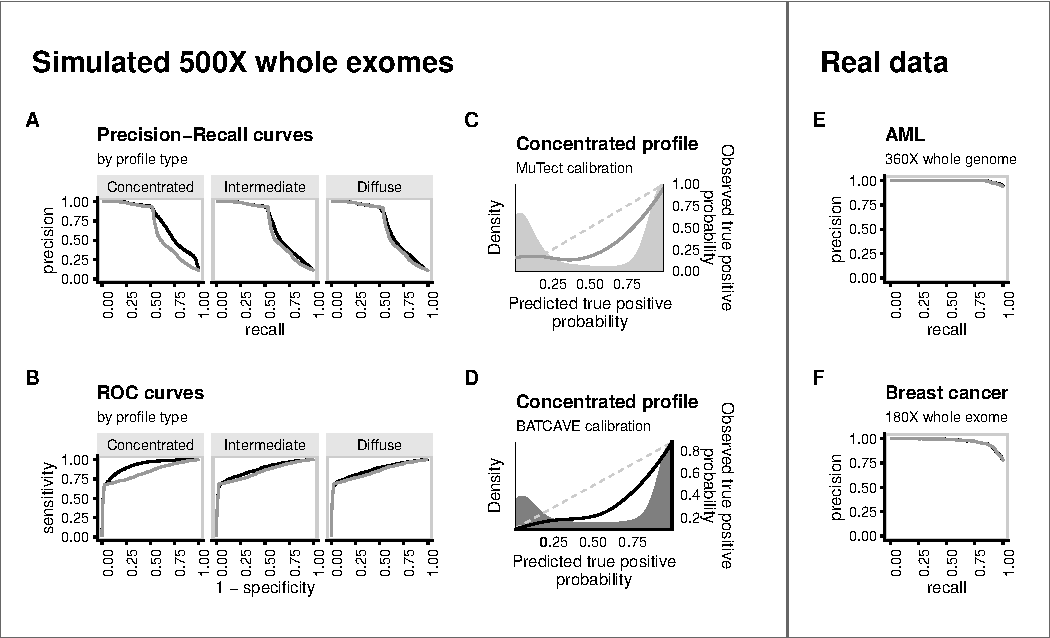
\includegraphics{figures/fig_wes.pdf}
    \end{center}
    \caption{Model performance on 500X simulated whole exome.
    \textbf{(a)} Precision recall curves and \textbf{(c)} Receiver operating characteristic curves for 3 mutation signatures.
    Distribution of estimated true positive probabilities for true positive (top) and true negative (bottom) variants for \textbf{b)} the MuTect model and \textbf{d)} the \batcave model.
    A perfectly calibrated model would generate the diagonal line.}
  \label{NAR-wes_fig}
  \end{figure*}

\section{RESULTS}
We designed \batcave as a post-call variant evaluation algorithm to be used with MuTect (Versions 1.1.7 or $>$2.0) \cite{Cibulskis2013}.
The algorithm is effecient, processing 22,000 variants per second on a typical iMac desktop computer, which corresponds to 100 seconds to process a 500X exome and 2000 seconds for a 100X whole genome.
MuTect is widely used, has state of the art sensitivity and specificity, and includes numerous heuristic filters and alignment adjustments that reduce the prevalence of sequencing errors in results \cite{Griffith2015}.
\batcave takes the output from MuTect, extracts the log-likelihood ratio for each potential variant site, and uses that ratio to separate the potential sites in to high-confidence and low-confidence groups.
The mutation profile is computed from the high confidence sites, and the posterior probability of mutation is recomputed for all sites as described in Materials and Methods.

\begin{figure}
  \begin{center}
  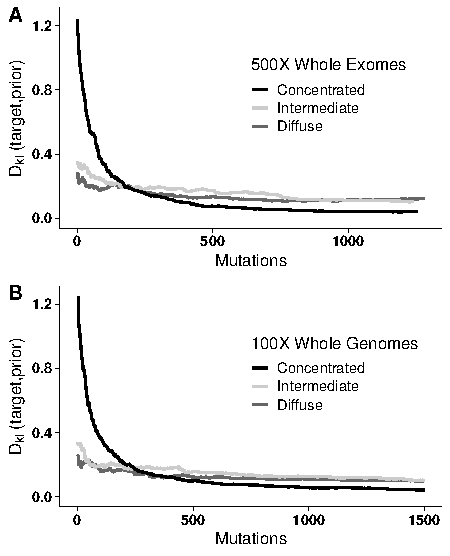
\includegraphics{figures/kl_only.pdf}
  \end{center}
  \caption{KL divergence between the estimated profile ($\boldsymbol{\pi}$) and the simulated mutation profile for \textbf{(f)} Whole exomes and \textbf{(g)} whole genomes.
  The estimated mutation profile converges quickly to the target as the number of mutations evaluated rises.}
\label{NAR-kl_fig}
\end{figure}

\subsection{Convergence of the site-specific prior to the data generating distribution}
The context-dependent prior probability of mutation, the heart of \batcave, depends on the prior converging to a good representation of the data generating distribution within the set of high-confidence mutations.
We use the Kullback-Leibler (KL) divergence as a measure of the distance (or entropy difference) between the estimated prior and the actual simulated data generating distribution.
In Figure \ref{NAR-kl_fig} we order mutations by descending MuTect probability value, and compute the KL divergence between the prior after adding each mutation and the data generating distribution.
For both whole exome and whole genome the prior converges to the data generating distribution easily within the number of available high-confidence mutations, which for the \citet{Griffith2015} leukemia is over 17000, and for our simulated data sets ranges between 1500 and 5000.




\subsection{Simulated data}
We generated six different tumor/normal pairs of two types, 3 each of 100X depth whole genomes and 500X whole exomes.
For each of the two types we simulated tumors with variants drawn from three different mutation profiles chosen to resemble melanoma (concentrated), a lung cancer (intermediate), and a BRCA-driven breast cancer (diffuse)  as described in Materials \& Methods and Figure \ref{NAR-sigfig}.
These 6 simulated tumor/normal pairs were used to assess the effect of sequencing depth and mutation profile type on the results obtained from \batcave.



We assessed classification performance with both the area under the ROC curve and the area under the precision-recall curve, because the classes here are unbalanced (approximately 5 to 1 ratio of false to true variants in our simulated data).
By both metrics \batcave outperforms MuTect (Figure \ref{NAR-wes_fig} \textbf{a} and \textbf{c}, and Table \ref{table:01}).
The extent to which \batcave outperforms is dependent on both the sequencing depth and the level of concentration of the mutation signature.
Deeper sequencing and more concentrated mutation signatures increase the performance advantage of \batcave. 

The estimated mutation rate is approximately $3\cdot10^{-7}$ for all simulated tumors (Table \ref{table:01}).
We note that the effective mutation rate is lower than the simulated rate of $3\cdot10^{-6}$.
In this case the lower effective rate is not due to normal contamination of the tumor sample, but the fact that \texttt{Bamsurgeon} has restrictions -- such as sequencing depth and quality -- that prevent 100\% of simulated variants from being inserted. 

We measured overall calibration performance using the Integrated Calibration Index (ICI) described in Methods \citep{Austin2019}.
The ICI is a measure of the difference between predicted and observed probabilities that is weighted by the empirical density of the predicted probabilities.
This is useful in our setting because the density of posterior probabilities tends to be strongly bi-modal.
A large fraction of true negative variants have posterior probabilities of less than $10{-4}$, which is a probability far below any threshold that is meaningful, we evaluate calibration only on variants with posterior probability greater than .01.
As we can see in Figure \ref{NAR-wes_fig} \textbf{b} and \textbf{d}, \batcave tends to increase posterior probabilities of low probability but true variants (density curves) while decreasing the probability of low probability but false variants (density not shown).
For 500X tumors the calibration of \batcave is better across the full spectrum of posterior probabilities, while for 100X whole genomes the calibration is slightly worse (Figure \ref{NAR-wgs_fig} and Table \ref{table:01}).
This effect is likely due to the fact that there are simply very few low probability true positive variants in tumor sequenced to 100X depth.
As with all other metrics, the benefit of \batcave increases as the concentration of the mutation profile increases, and as sequencing depth increases.

Figure \ref{NAR-ppv_fig} takes a consolidated view of classification accuracy and calibration for 500X whole exomes in the portion of the posterior probability distribution relevant to clinicians and researchers.
For any probability between 60 and 90\% \batcave is better calibrated than Mutect.
Essentially, for any posterior probability above 70\% MuTect has a false positive rate around 8\%, while \batcave has a false positive rate that increases as posterior probability decreases.
The cost of this compression is recall, which is 3-5\% better than MuTect at 95\% posterior probability, and 3-7\% better at 90\%, depending on muation profile concentration.
At any posterior probability \batcave returns a larger fraction of all positive calls than MuTect.
Figure \ref{NAR-ppv_wgs_fig} shows results for 100X whole genomes, where the results are similar for precision.
Note that recall never improves because the uncalled true positive variants are below the threshold of detection for any reasonable level of false positive calls.

\subsection{Real tumor data.}
We utilized two real data sets.
In each, deep sequencing and variant validation were performed with the specific purpose of evaluating tumor variant calling pipelines.
These are among a very small number of tumors which have been sequenced at high depth, and for which variant validation was undertaken.
\citet{Griffith2015} sequenced the whole genome of an acute myeloid leukemia (AML) primary tumor to a depth of $>360\mathrm{X}$, and used targeted sequencing to validate nearly 200,000 mutations.
We downloaded aligned reads for this tumor, and called variants with MuTect 1.1.7 as described in Materials \& Methods.
We estimated a per-base mutation rate for this tumor of $3\cdot10^{-8}$, which is line with the mutation rates generally considered normal in AML.
The area under the precision-recall curve is essentially identical (.995 \& .996) for MuTect and \batcave (Figure \ref{NAR-wes_fig} \textbf{a} and \textbf{b} and Table \ref{table:01}).

\citet{Shi2018} performed multi-region whole exome sequencing on 6 individual breast tumors to a mean target sequencing depth of $160\mathrm{X}$, and validated all variants identified by three different variant calling pipelines.
We downloaded aligned reads for this tumor, and called variants with MuTect 1.1.7 as described in Materials \& Methods.
We estimated a per-base mutation rate for this tumor of $3\cdot10^{-8}$, and the area under the precision-recall curve is identical (.972) for MuTect and \batcave (Figure \ref{NAR-wes_fig} \textbf{b} and Table \ref{table:01}).

We report only precision-recall comparisons for real tumor data because in both cases the "gold" standard data sets consist of variants that were "called" by one or more variant detection pipelines, and confirmed to be present or absent \cite{Griffith2015,Shi2018}.
These mutations are in some sense \textit{easy} to call, since at least one variant caller did in fact call them.
At the same time, there is no way to compute true and false negative fractions for these data sets.
As such, it is not surprising that the performance of MuTect and \batcave are similar because the universe of variants under consideration in these experiments are by definition "callable" by at least one variant detection pipeline, and MuTect is among the most sensitive and specific variant callers \cite{Griffith2015,Cibulskis2013}.

\begin{figure}
  \begin{center}
  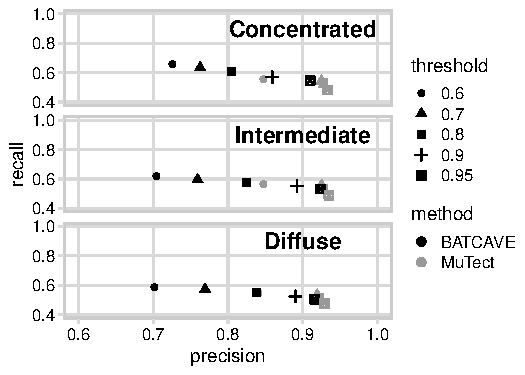
\includegraphics{figures/ppv_wes.pdf}
  \end{center}
  \caption{Model performance on 500X simulated whole exome. 
  Positive predictive values vs. Recall for three different probability cutoffs. 
  Note the restricted axes to improve readability of points}
\label{NAR-ppv_fig}
\end{figure}



\section{DISCUSSION}
 
Deep sequencing is necessary to measure quantities such as intra-tumor heterogeneity \cite{Shi2018}, sub-clonal presence of driver and resistance alleles \cite{Griffith2015}, and the mutational landscape of cancer in general \cite{Zehir2017}.  
As \citet{Griffith2015} show, whole genome sequencing at approx. 350X average depth requires combining calls from many variant calling algorithms, and then validating these calls via ultra-deep targeted sequencing. 
We believe that much of the need for multiple variant callers could be alleviated by improvements to the statistical model used to evaluate the evidence presented by the sequenced reads. 

\batcave is a post-call variant evalutation tool that uses MuTect output and the tumor-specific mutation profile to sharpen the posterior probability assigned to SNVs.
We demonstrated here that \batcave improves classification accuracy in synthetic data, leading to better more accurate variant calls at any posterior probability threshold.
Importantly, \batcave is better calibrated than MuTect at relevant probability thresholds, allowing researchers and clinicians to make informed choices about the trade-off between precision and recall.
We are unable to study calibration in real data, because complete false positive/true negative data for real data is not available. 
Deep sequencing experiments where a large random sample of uncalled potential variants, as well as a random sample of variant with no reads at all present, would give much-needed insight into the differences in statistical models in variant calling.

\batcave resembles an empirical Bayes approach, but is not really empirical Bayes.
In fact, variants are best described as sequential samples from a data generating distribution represented by the mutation profile.
Early mutations are classified with low error, while later mutations are classified with less certainty.
We show here that sequential updating of the dirichlet-multinomial posterior converges to the true data generating distribution using the set of early mutations.
Along with the assumption that tumor evolution is approximately neutral, this allows us to generate a tumor and site-specific that sharpens the classification and calibration of later mutations.
Thus, \batcave is best described as an algorithm trained on early mutations.

\bkmcomment{this needs more work}
We simulate tumors with three mutation profiles, and evaluate two real tumor data sets.
Among these performance is best with the most concentrated simulatin profile.
The intermediate and diffuse mutation profiles are designed to represent baseline or minimal profiles of Lung and Breast tumors respectively.
In fact, lung and breast tumors have heterogeneous mutation profiles with a wide range of levels of concentration.
The Acute Myeloid Leukemia we evaluated has a particularly diffuse profile, which is common for these tumors \cite{Alexandrov2019}.

The \batcave algorithm focuses on the tri-nucleotide context and substitution type, which has been shown to have a large effect on site-specific mutation rates \cite{Martincorena2015,Hollstein2017}.
There are, however, many other types of \textit{genomic context} which can effect local mutation rates including replication timing, expression level, and chromosome organization \cite{Buisson2019,Schuster-Bockler2012,Pleasance2010}.
\bkmcomment{what to say here? Are we acknowledging a weakness, or just observing there are other types?}
These could be very useful in computing a local or regional mutation rate, as opposed to the genome-wide but tumor-specific mutation rate used by \batcave.

We have chosen to implement \batcave as a post-calling algorithm for exclusive use with MuTect because MuTect presents a simple model and a well-tested set of heuristic filters.
However, the model is very general, and in principle there is no barrier to using the method with other variant callers.
For instance Strelka2, another widely used variant caller, computes a joint posterior probability over tumor and normal genotypes where the prior probability that the tumor carries a somatic mutation at a given site is set to a constant \cite{Kim2018}.
Modifying the algorithm to work with the Strelka statistical model would involve replacing the constant prior with a tumor and site-specific prior for each potential variant, exactly as we have done with MuTect.

The R implementation \texttt{batcaver} adds 1 second per 22,000 variants evaluated to a standard GATK best practices variant calling pipeline. 
The majority of the computational overhead in \batcave is associated with extracting the tri-nucleotide context for each potential variant site from the reference genome.
Since most variant callers are already walking the reference genome as part of the calling process, extracting the tri-nucleotide context simultaneously would dramatically reduce the computational overhead associated with implementing \batcave.

We hope that the availability of this algorithm will have a positive effect on the cost/benefit ratio of deeper sequencing in both research and clinical applications.
One size does not fit all with respect to the evidence threshold. 
Users are interested in true and false positive fractions, and users of different types will have different trade-offs in terms of precision and recall.
We present \batcave, and the R package \texttt{batcaver} to provide the user with a more accurate sense of these trade-offs.

% \section{CONCLUSION}
% \bkmcomment{I looked at a bunch of NAR methods papers, and none include a conclusions section, so I moved it to the last paragraph of discussion.}

\section{Software Availability}
\bkmcomment{working on this today}

github for source code

zenodo for figures, simulations

zenodo for package at time of bioarxiv

\section{ACKNOWLEDGEMENTS}

This work was supported by the National Science Foundation via Graduate Research Fellowship DGE-1143953 to BKM and \bkmcomment{RNG NIH}.
The authors would like to thank Professor Edward J. Bedrick for fruitful discussions about the statistical model.


\subsubsection{Conflict of interest statement.} None declared.

\bibliography{caller_paper}

\beginsupplement
\section{Supplememtary Figures}

\begin{figure}[b]
  \begin{center}
  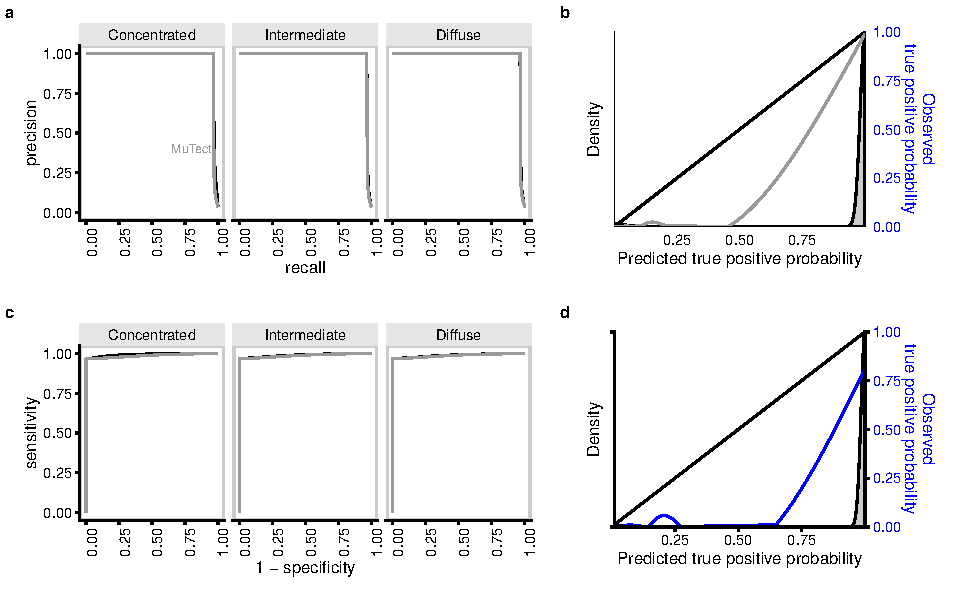
\includegraphics{figures/fig_wgs.pdf}
  \end{center}
  \caption{Model performance on 100X simulated whole genome.
  \textbf{(a)} Precision recall curves and \textbf{(c)} Reciever operating characteristic curves for 3 mutation signatures.
  Distribution of estimated true positive probabilities for true positive  variants for \textbf{b)} the MuTect model and \textbf{d)} the \batcave model.
  A perfectly calibrated model would generate the diagonal line.}
\label{NAR-wgs_fig}
\end{figure}



\clearpage
\begin{figure}
  \begin{center}
  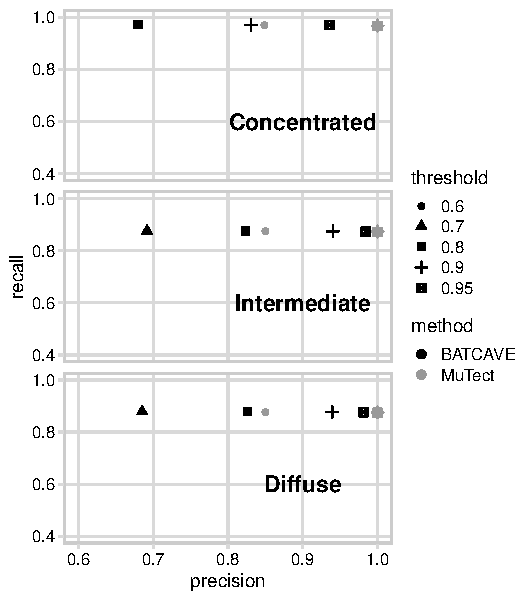
\includegraphics{figures/ppv_wgs.pdf}
  \end{center}
  \caption{Model performance on 100X simulated whole genome. 
  Positive predictive values vs. Recall for three different probability cutoffs. 
  Note the restricted axes to improve readability of points.}
\label{NAR-ppv_wgs_fig}
\end{figure}

\section{Supplememtary Table}

\begin{table}[b]
  \tableparts{%
  \caption{Performance characteristics as measured for all data sets.}
  \label{table:01}%
  }{%
  \begin{tabular*}{\textwidth}{@{}lllllllll@{}}
  \toprule
  Depth & Mutation profile & $\mu$ & AUROC & & AUPRC & & ICI & 
  \\
  & & (estimated) & MuTect & \batcave & MuTect & \batcave & MuTect & \batcave
  \\
  \colrule
  100X whole genome & Concentrated & 3.6e-7 & .987 & .993 & .972 & .975 & .117 & .287
  \\
  100X whole genome & Intermediate & 3.2e-7 & .987 & .989 & .972 & .973 & .118 & .214
  \\
  100X whole genome & Diffuse & 3.2e-7 & .988 & .989 & .971 & .973 & .120 & .219
  \\
  500X whole exome & Concentrated & 3.6e-7 & .848 & .929 & .674 & .758 & .138 & .109
  \\
  500X whole exome & Intermediate & 3.6e-7 & .847 & .881 & .677 & .706 & .108 & .112 
  \\
  500X whole exome & Diffuse & 3.6e-7 & .850 & .873 & .676 & .698 & .105 & .116
  \\
  \citet{Griffith2015} & Actual & 3.6e-8 & -- & -- & .995 & .996 & -- & --
  \\
  \citet{Shi2018} & Actual & 3.6e-8 & -- & -- & .972 & .972 & -- & --
  \\
  \botrule
  \end{tabular*}%
  }
  {$\mu$ = per-base mutation rate, AUROC/AUPRC = area under ROC/PRC curve, ICI = Integrated calibration index.}
 \end{table}

\end{document}

